\documentclass[UTF8]{ctexart}
%\usepackage[margin=1.5cm]{geometry} %設定四個邊界皆為 1.5 cm
\usepackage[left=2cm, right=2cm, top=1.5cm, bottom=1.2cm]{geometry} %設定左邊界2cm,右邊界2cm,上邊界1.5cm, 下邊界 1.2cm
\setlength{\parindent}{0pt} %開頭不縮排

\usepackage{mathtools}

\usepackage{pgfplots}       % 使用pgfplots繪圖工具包
\pgfplotsset{width=7cm,compat=1.13} % 圖片繪制的寬度是7cm,使用的pgfplots版本是1.13

\usepackage{graphicx} %插入圖片函式庫
\usepackage{caption}
\usepackage{subfigure}
\usepackage{verbatim}  % 多行註解需使用verbatim package

%\usepackage{comment} %多行註解函式庫

\begin{document}
\begin{CJK*}{UTF8}{song}
%\thispagestyle{empty} %首頁頁碼空白
\setlength{\baselineskip}{20pt} %全部行距皆為 30 points

%標題
\begin{center}
\begin{LARGE} 
\textbf{Transport Measurements Experiment 結報} \\
\end{LARGE} 
\begin{large} 
B5組 0412107 陳麒升、0412001 陳勁宇  
\end{large}
\end{center}

%%%%%%%%%%%%%%%<1頁%%%%%%%%%%%%%%%%%%
%動機
\begin{large}
\textbf{1.實驗動機與目的:} \\
\end{large}
實驗各種元件於不同溫度下對電阻的關係。
 \\
 \\
%
% 你認為或發現的實驗操作重點方式,條列式 ≤ 五項
\begin{large}
\textbf{2.實驗操作重點方式:} \\
\end{large}
◆於實驗操作方面我們組別認為需要注意的有: \\
(1) 對於非半導體之金屬元件,量測不同溫度下不同金屬元件的電阻數值,並做電阻-溫度關係圖。 \\
(2) 對於半導體元件,量測不同溫度下不同元件之電壓數值,並做電流-電壓圖。 \\
(3) 於實驗期間,宜將電源供應器上之電流檔位轉至最大(以防隨著電壓改變的電流大於預設檔位)再依據實驗要求調整電壓。 \\

%%%%%%%%%%%%%%%%%%%%%%%%%%%%%%%%%%%%%%


%%%%%%%%%%%%%%%2~5頁%%%%%%%%%%%%%%%%%%
% 附課堂上操作的原始數據資料等
\begin{large}
\textbf{3.實驗raw data:} \\
\end{large} 
一、金屬元件: \\
C代表Carbon layer resistor,Met代表Metallic layer resistor,NTC代表Negative Temperature Coefficient thermistor,PTC代表Positive Temperature Coefficient thermistor。  \\ 
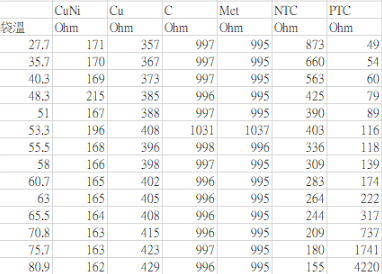
\includegraphics[width = 0.5\textwidth]{allRes.png} \\
\newpage

二、半導體元件: \\
(1) $29^{\circ}C$ : \\
%◆$Ge$ : \\
%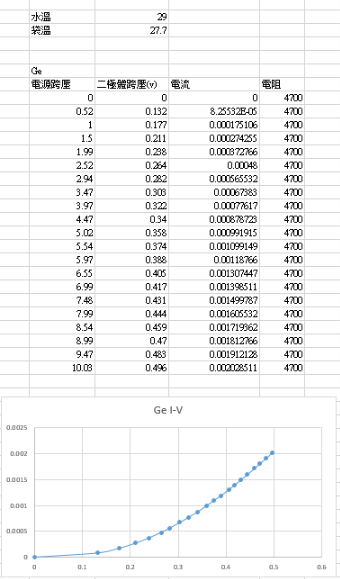
\includegraphics[width = 0.3\textwidth]{29ge.png} \\
%◆$Si$ : \\
%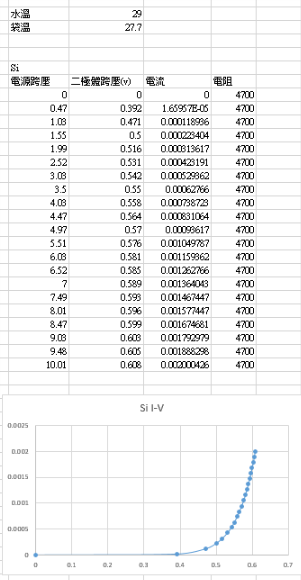
\includegraphics[width = 0.3\textwidth]{29si.png} \\


\begin{minipage}[t]{0.48\textwidth}
\centering %子圖居中
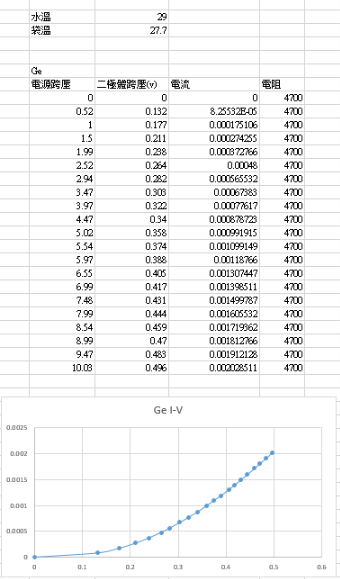
\includegraphics[width = 0.6\textwidth]{29ge.png}
%\caption{$Ge$}
\end{minipage} %如果minipage間有空行則圖片不會並排
\begin{minipage}[t]{0.48\textwidth}
\centering
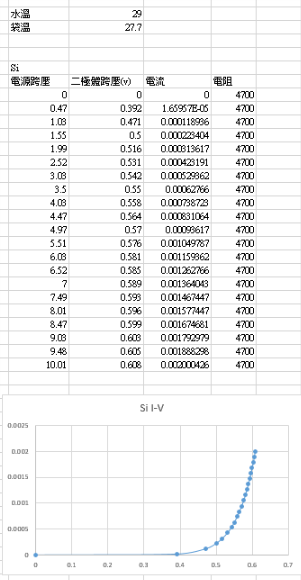
\includegraphics[width = 0.6\textwidth]{29si.png}
%\caption{$Si$}
\end{minipage}
 \\

\begin{minipage}[t]{0.48\textwidth}
\centering
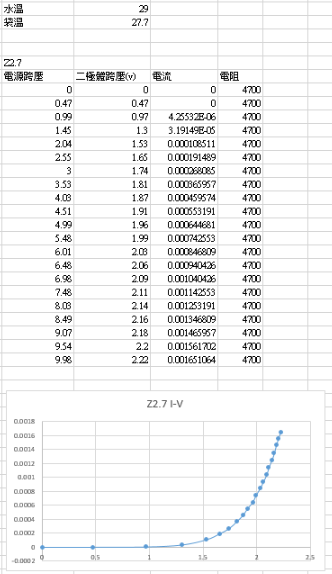
\includegraphics[width = 0.6\textwidth]{29z27.png}
%\caption{$z2.7$}
\end{minipage}
\begin{minipage}[t]{0.48\textwidth}
\centering
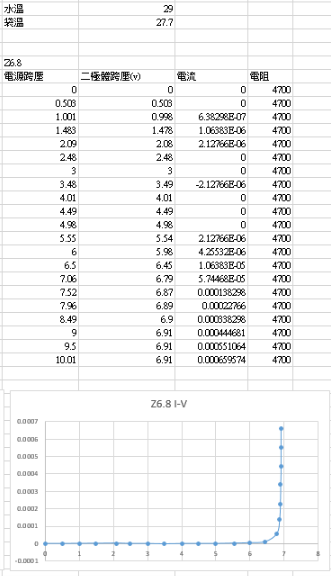
\includegraphics[width = 0.6\textwidth]{29z68.png}
%\caption{$z6.5$}
\end{minipage}




\begin{comment}  % 註解開始
%\newpage %強制分頁
◆$Z6.8$ : \\
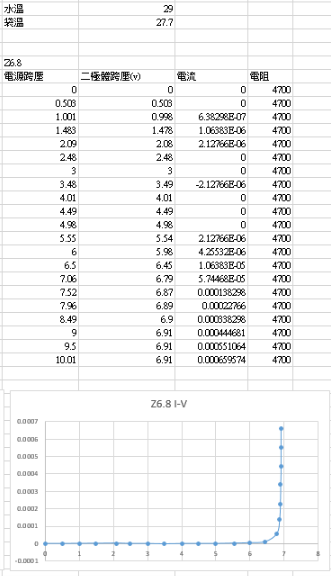
\includegraphics[width = 0.3\textwidth]{29z68.png} \\

◆$Z2.7$ : \\
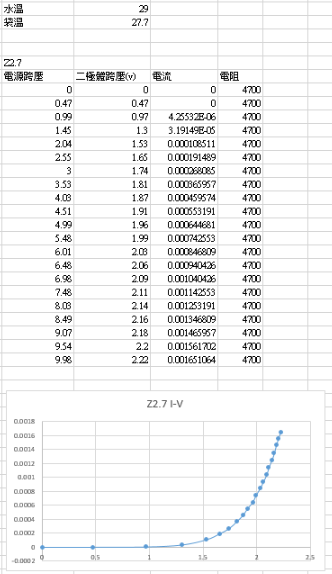
\includegraphics[width = 0.3\textwidth]{29z27.png} \\
\\

\newpage %強制分頁


(2) $45^{\circ}C$ : \\
◆$Ge$ : \\
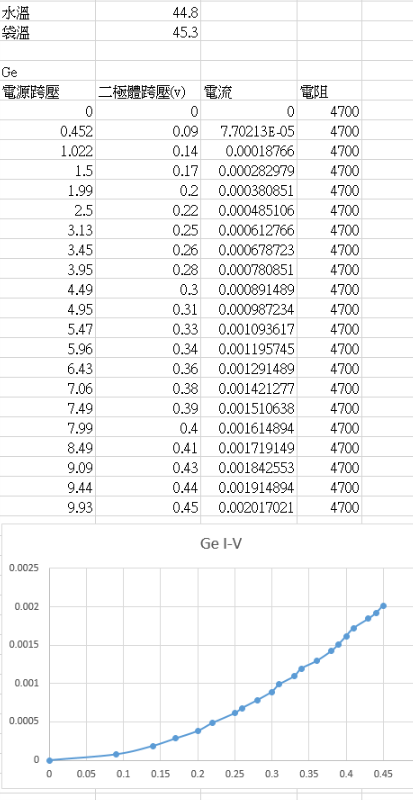
\includegraphics[width = 0.3\textwidth]{45ge.png} \\

◆$Si$: \\
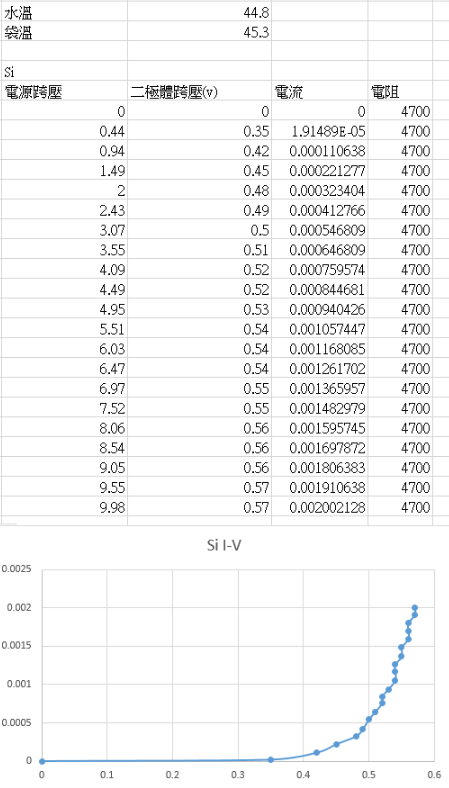
\includegraphics[width = 0.3\textwidth]{45si.png} \\

◆$C_{2}H_{5}OH (95\%)$ : \\
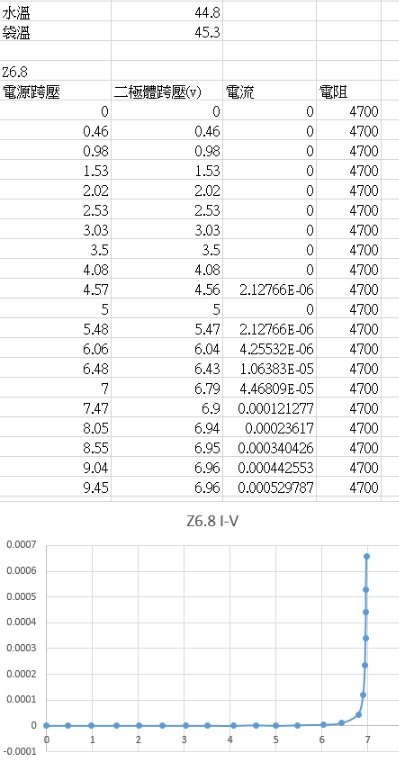
\includegraphics[width = 0.3\textwidth]{45z68.png} \\
\\

接下來之附件為附上方格紙的實驗光斑raw data紀錄結果。

\newpage
\end{comment}  % 註解結尾
\newpage

(2) $45^{\circ}C$ : \\

\begin{minipage}[t]{0.48\textwidth}
\centering %子圖居中
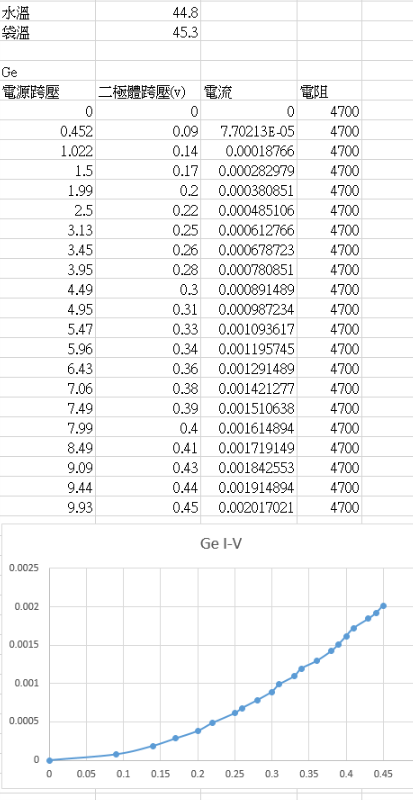
\includegraphics[width = 0.6\textwidth]{45ge.png}
%\caption{$Ge$}
\end{minipage} %如果minipage間有空行則圖片不會並排
\begin{minipage}[t]{0.48\textwidth}
\centering
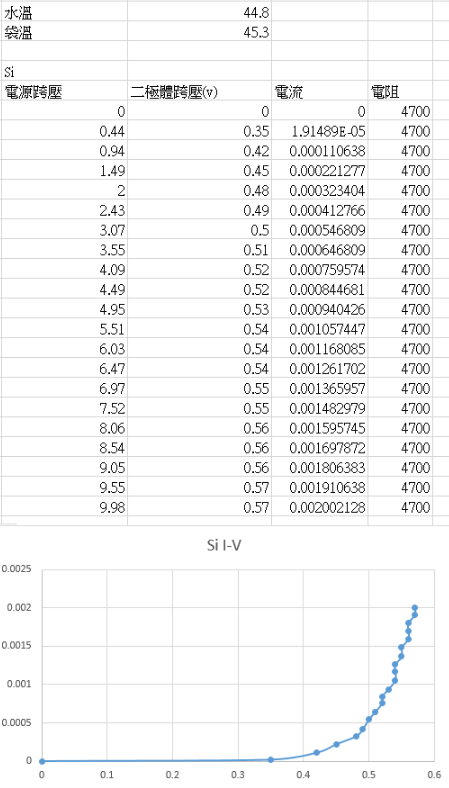
\includegraphics[width = 0.6\textwidth]{45si.png}
%\caption{$Si$}
\end{minipage}
 \\

\begin{minipage}[t]{0.48\textwidth}
\centering
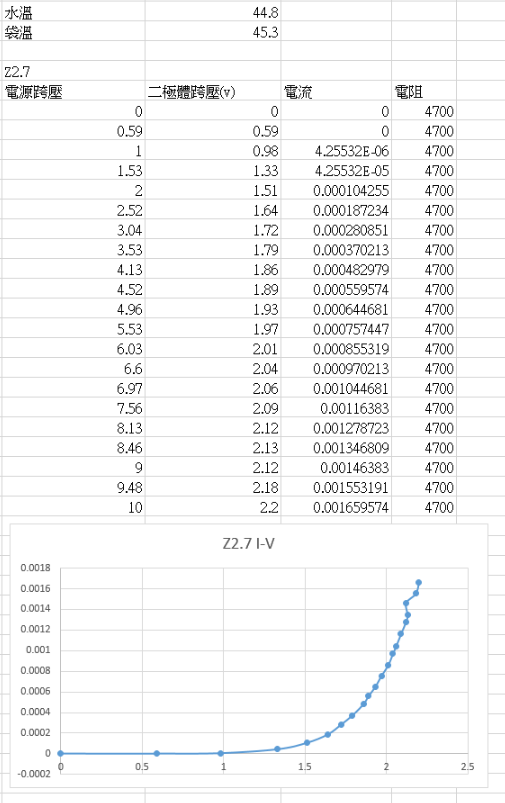
\includegraphics[width = 0.6\textwidth]{45z27.png}
%\caption{$z2.7$}
\end{minipage}
\begin{minipage}[t]{0.48\textwidth}
\centering
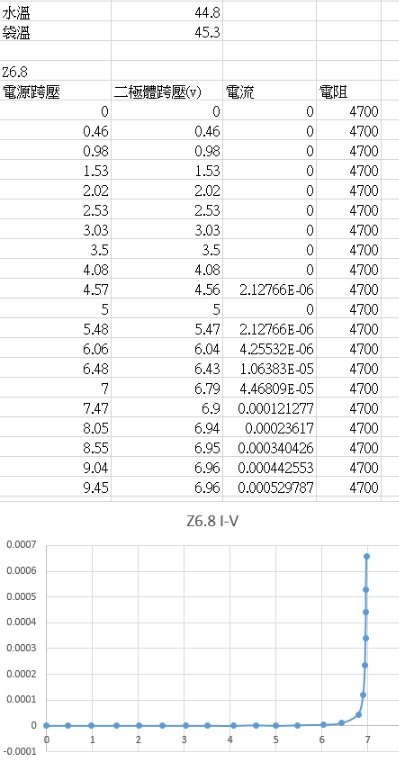
\includegraphics[width = 0.6\textwidth]{45z68.png}
%\caption{$z6.5$}
\end{minipage}
\newpage

(3) $65^{\circ}C$ : \\

\begin{minipage}[t]{0.48\textwidth}
\centering %子圖居中
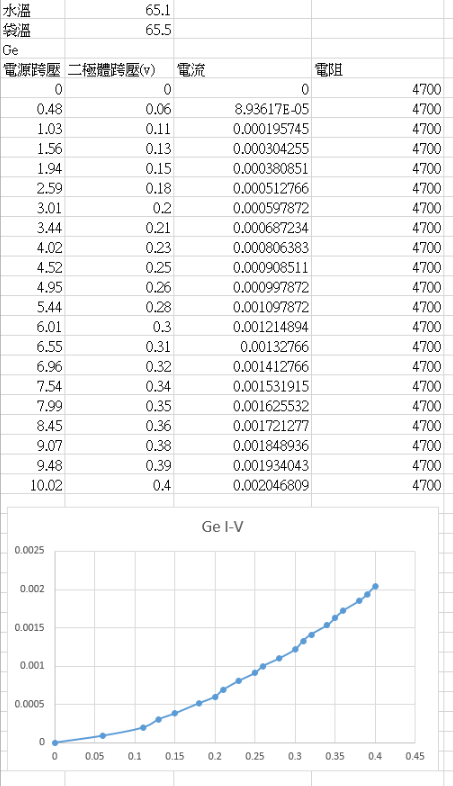
\includegraphics[width = 0.6\textwidth]{65ge.png}
%\caption{$Ge$}
\end{minipage} %如果minipage間有空行則圖片不會並排
\begin{minipage}[t]{0.48\textwidth}
\centering
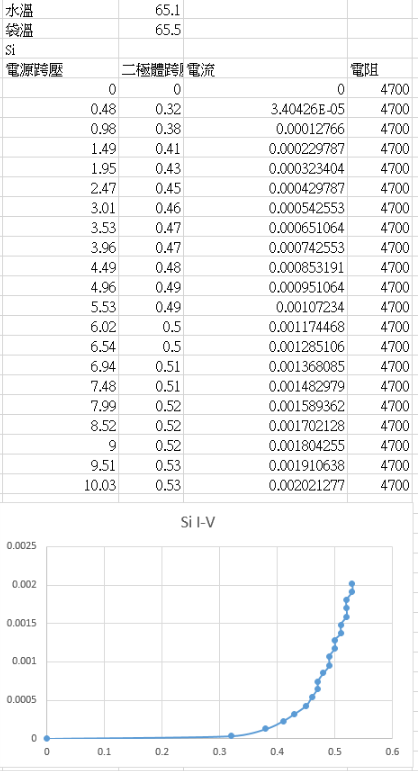
\includegraphics[width = 0.6\textwidth]{65si.png}
%\caption{$Si$}
\end{minipage}
 \\

\begin{minipage}[t]{0.48\textwidth}
\centering
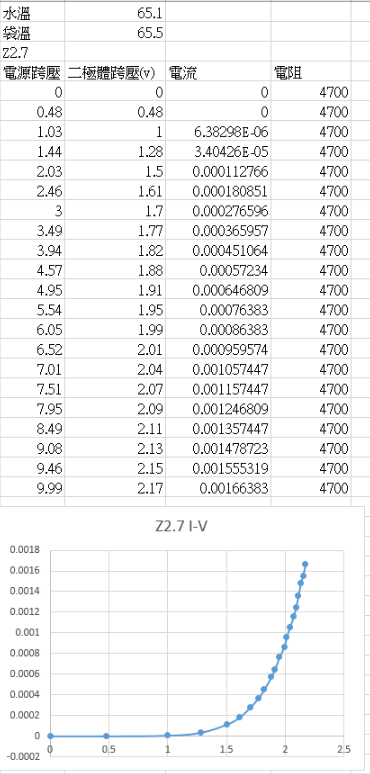
\includegraphics[width = 0.6\textwidth]{65z27.png}
%\caption{$z2.7$}
\end{minipage}
\begin{minipage}[t]{0.48\textwidth}
\centering
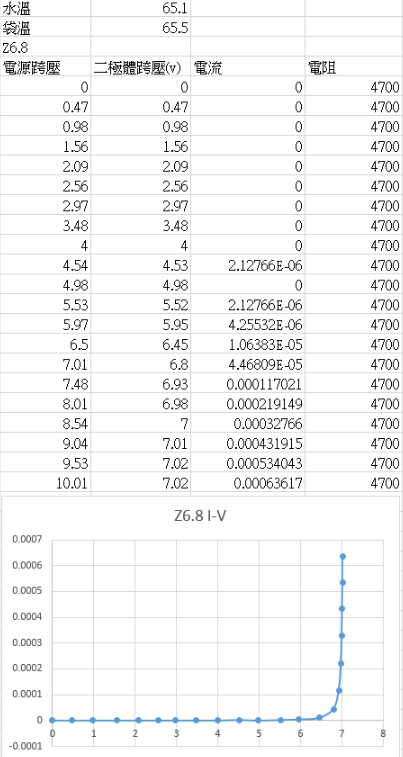
\includegraphics[width = 0.6\textwidth]{65z68.png}
%\caption{$z6.5$}
\end{minipage}
\newpage

(4) $80^{\circ}C$ : \\

\begin{minipage}[t]{0.48\textwidth}
\centering %子圖居中
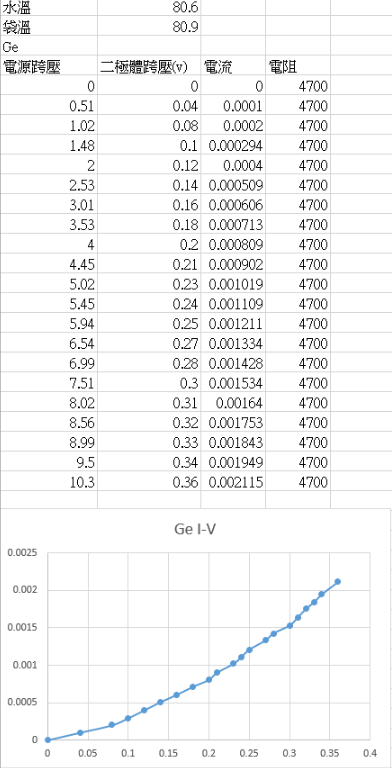
\includegraphics[width = 0.6\textwidth]{80ge.png}
%\caption{$Ge$}
\end{minipage} %如果minipage間有空行則圖片不會並排
\begin{minipage}[t]{0.48\textwidth}
\centering
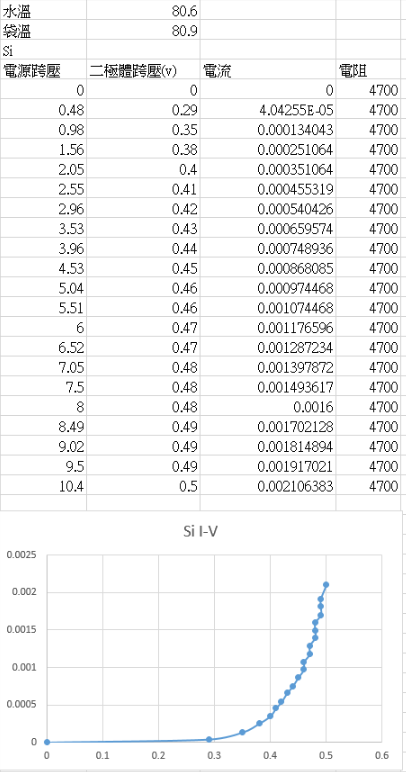
\includegraphics[width = 0.6\textwidth]{80si.png}
%\caption{$Si$}
\end{minipage}
 \\

\begin{minipage}[t]{0.48\textwidth}
\centering
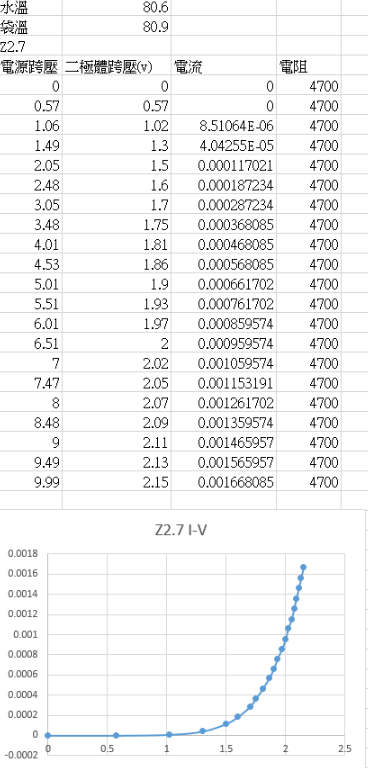
\includegraphics[width = 0.6\textwidth]{80z27.png}
%\caption{$z2.7$}
\end{minipage}
\begin{minipage}[t]{0.48\textwidth}
\centering
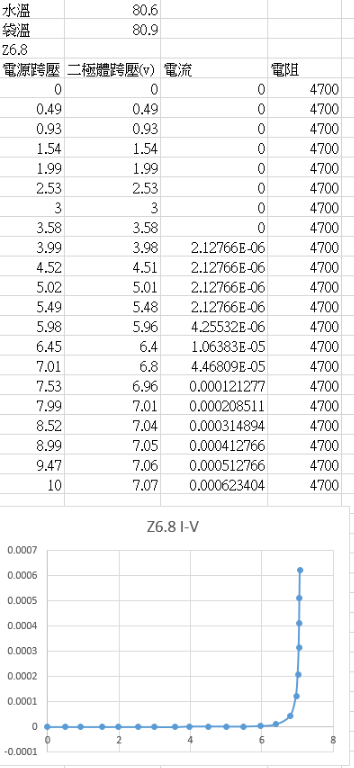
\includegraphics[width = 0.6\textwidth]{80z68.png}
%\caption{$z6.5$}
\end{minipage}
\newpage

% 資料分析數據整理
\begin{large}
\textbf{4.資料分析數據整理: } \\
\end{large}
一、金屬元件 :  \\
下圖為各元件於不同溫度下對電阻值作圖: \\
\includegraphics[width = 0.6\textwidth]{ohmt.png} \\
由圖中可以看到,$Cu$、$CuNi$、$Met$、$C$圖形大致成線性,此結果符合資料中 $\alpha$大致於$10^{-3}$以下。而$PTC$、$NTC$則維持指數關係,$\alpha$較大,亦符合理論值所預期。 \\
 \\
二、半導體元件 :  \\
1. $Ge$ 於不同溫度下之電流對電壓關係作圖 :  \\
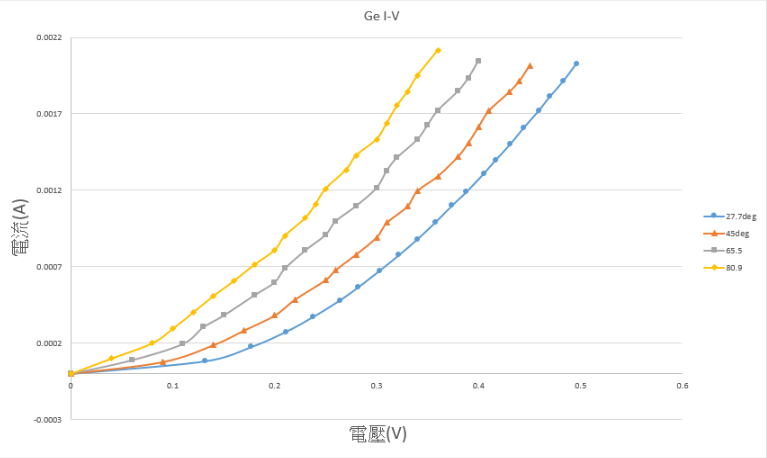
\includegraphics[width = 0.7\textwidth]{geAll.png} \\
由圖中可以看到鍺隨著溫度升高,曲線會漸漸向左移動,即在相同電壓下,越高溫會使鍺中帶電載子數增加,使之能產生較低溫時為大的電流,並且使的曲線切線斜率(即電導)$I/V$變大。 \\
\newpage

2. $Si$ 於不同溫度下之電流對電壓關係作圖 : \\
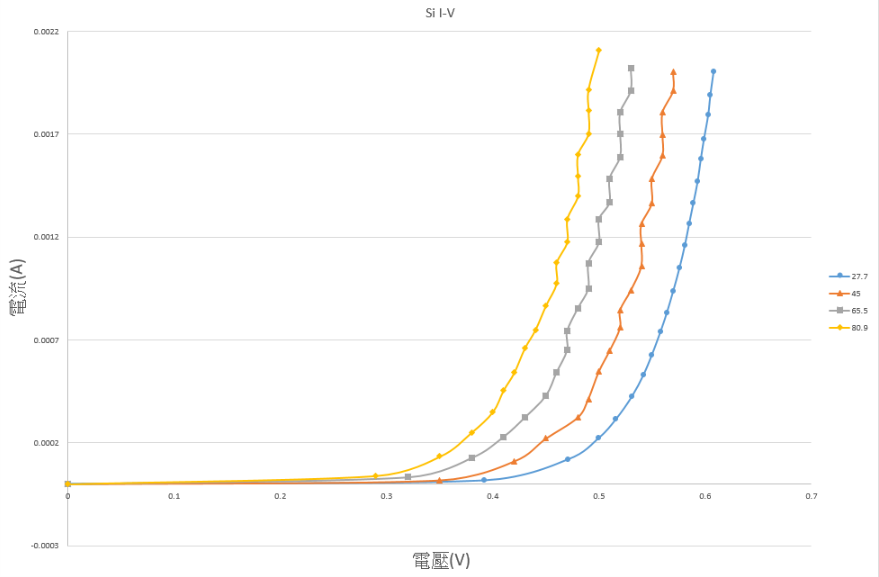
\includegraphics[width = 0.7\textwidth]{siAll.png} \\
由圖中可以看到矽隨著溫度升高,曲線會漸漸向左移動,即在相同電壓下,越高溫會使矽中帶電載子數增加,使之能產生較低溫時為大的電流,並且使的曲線切線斜率(即電導)$I/V$變大。 此趨勢結果與鍺相近,不過矽較鍺切線斜率更大,即在相同電流、相同溫度的情況下矽電壓較鍺為大。 此一現象可從元素週期表上得到解釋,矽與鍺同是$IV A$族元素,而矽之原子序洽較鍺小一個週期,因此在相同電流、相同溫度的情況下矽電壓較鍺為大。\\

3. $Z_{6.8}$ 於不同溫度下之電流對電壓關係作圖 :  \\
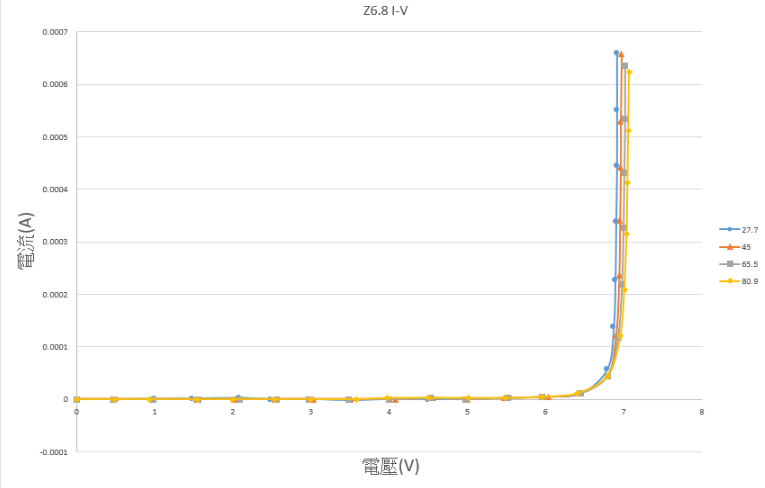
\includegraphics[width = 0.7\textwidth]{z68All.png} \\
\newpage

4. $Z_{2.7}$ 於不同溫度下之電流對電壓關係作圖 :  \\
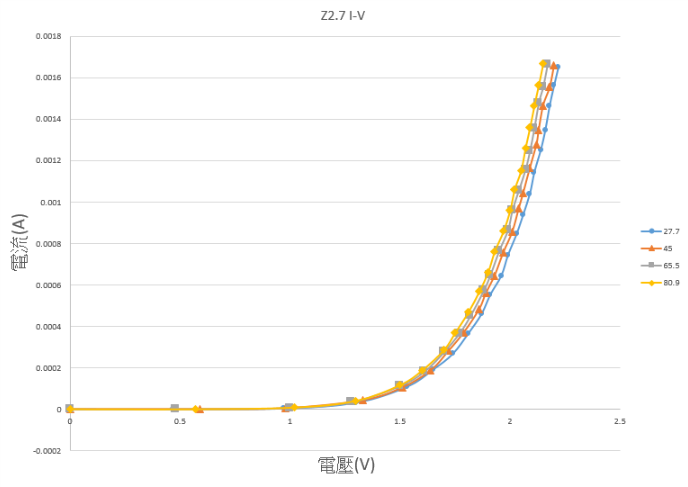
\includegraphics[width = 0.7\textwidth]{z27All.png} \\
我們將3.和4.一同相互比較。所謂的$Z$所指的是Zener diode,$Z_{6.8}$ 猜測即為崩潰電壓約莫在$6.8V$的Zener diode,而$Z_{2.7}$ 猜測即為崩潰電壓約莫在$2.7V$的Zener diode。 從上2圖可以得知,$Z_{6.8}$ 的崩潰電壓大約在於$6.8V$左右,並隨溫度上升而增大,因此可知 $Z_{6.8}$ 是由avalanche effect所產生 ; 而$Z_{2.7}$的崩潰電壓大約從$1.5V$左右開始一路到$2.5V$左右傾斜趨勢都尚未停歇,假設Zener diode $Z_{2.7}$之崩潰電壓中心點在$2.7V$,則預計其崩潰電壓之極大值大約在$4V$左右,並隨溫度上升而減小,因此可知 $Z_{2.7}$ 是由Zener effect所產生。\\

%%%%%%%%%%%%%%%%%%%%%%%%%%%%%%%%%%%%%%%

%%%%%%%%%%%%%%1~2頁%%%%%%%%%%%%%%%%%%

% 分析結果,系統誤差來源,數據或方式上的討論 等等,結論 (含問題回答或思考)
\begin{large}
\textbf{5.分析結果與誤差來源討論 :} \\
\end{large}
(1) 於金屬元件的數據中,在$53.3^{\circ}C$ 所有元件均有向上突起的小型peak,此peak破壞理論上應該線性的$Ohm-T$ 線性關係,依照推論有可能是在那時水溫和袋溫並未達到熱平衡所致。 \\


\begin{comment}  % 註解開始
% 如何改進(可有可無,若有請討論原因)
\begin{large}
\textbf{6.如何改進實驗: } \\
\end{large}


 \\
\newpage
\end{comment}  % 註解結尾


%列出猜考資料,各成員對此結報貢獻在何處
\begin{large}
\textbf{6.Reference: } \\
\end{large}
(1) e3上之實驗講義, "Transport Measurements", 2018 \\
 \\


\begin{large}
\textbf{7.組員貢獻分布: } \\
\end{large}
所有實驗與結報數據分析討論均是我們同組2人共同完成。 \\
(此次結報之~\LaTeX{} 格式繕打為 0412107 陳麒升負責 )

%$\sum_{i=1}^{n} f(x)$

\end{CJK*}
\end{document}